\chapter{Project Analysis}
\label{chap:prjan}

As in chapter~\ref{chap:intro}, the creation of a full ETSI MANO compliant
architecture, following the suggestions described in RFC 7665, require the
integration of multiple tools (some of them have been already briefly introduced
in~\ref{chap:intro}). The tools were chosen after their analysis, where pro and
cons have been studied and compared to the necessity of this thesis. Since the
project has been developed with the cloud provided by the University of Padua,
Openstack (which a product analysis can be found later
in~\ref{chap:prjan:sec:openstack}) has been used as base for our deployments.

\section{Architecture overview}

During the test-bed development the software architecture diverged from the
original one, experiencing different evolutions and modifications.

\subsection{VIBES architectural description}

In the original VIBES architectural design, based on leveraging virtualization
technologies, is possible to identify different macro-components, each of these
specialized in fulfilling a specific goal. For the ETSI standards, the Network
Function Virtualization (NFV) design should be composed as follows:
\begin{figure}[t]
 \centering 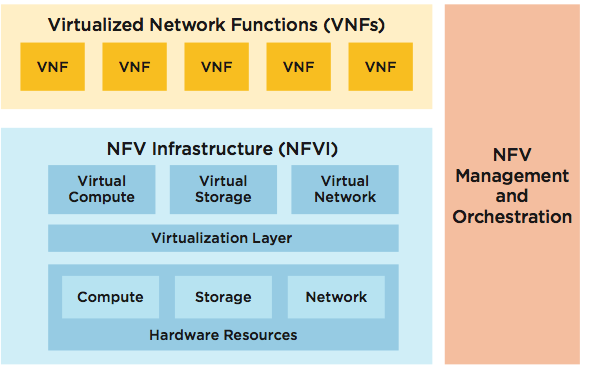
\includegraphics[scale=2]{etsi_arch}
 \caption{A schematic image representing the high level NFV architecture
   proposed by ESA.}
 \label{chap:prjan:img:etsi_arch}
\end{figure}

\begin{itemize}
 \item \textbf{Network Function Virtualization Infrastructure (NFVI)}: it's the
   heart of the whole computation component, and here three sub-domains can be
   identified: \todo{Expand this section}
\begin{itemize} 
 \item \textbf{Hyper-visor domain} that is composed of the Virtual Compute, the
   Virtual Storage, and the Virtualization Layer. These components are used to
   virtualize the computational and storage resources, providing a layer for
   accessing it.
 \item \textbf{Compute domain} composed by the Physical Compute and the Physical
   Storage. These are the real resources which are virtualized via software.
 \item \textbf{Infrastructure domain} which has the Physical Network, and its
   virtualized counterpart as made available by the Virtualization Layer.
\end{itemize}

In conventional virtualization systems these resources are usually separated
from the host operating system, providing better isolation but worst
performance. The ETSI infrastructure, instead, tries with container
virtualization technology to push for a better NFV responsiveness, removing the
additional operating system (called ``guest'' OS) required by the usual
hyper-visor-oriented approach.

To realize the required components, specific tools were suggested in the VNF
technical proposal: regarding the NFV (network infrastructure) domain
Docker-Compose was proposed as a viable solution, while to store PEP instances
docker swarm was described as a possible candidate.

We performed an accurate analysis of the tools chosen based on their maturity,
on the community and on the technical support offered (e.g. user manuals,
developer documentation), which, at the end, committed us to choose different
tools from the suggested ones. A detailed description of the architectural
implementation can be found in chapter~\ref{chap:archimpl}.\todo{Include prof.
  survey about community components here}

\item \textbf{VNFs} this are the core components that perform packets
  manipulation. This components are design to be lightweight services able to
  elaborate a great amount of packets per seconds. Manipulation can be of two
  typologies: stateful or stateless. In the first case, a state is maintained,
  and the VNF can perform heuristics about data coming through it (especially
  useful to detect patterns in the data flow, e.g. DDos attacks). In the second
  case, no state is maintained, and every packet is treated without any
  particular assumption. Following the RFC 7665, the VNF are also called Service
  Function (SF)\footnote{From now on the two terminologies will be use in a
    interchangeable way~\cite{medhat2017service}.}. Additional information can
  be found in Section~\ref{chap:prjan:sfc}.

\item \textbf{NFV Management and Orchestration (MANO)} also known as NFV
  Orchestrator (NFVO) is responsible for the end-to-end management and
  orchestration of network services (NS), also called SFC. The MANO has
  different responsibilities, such as managing the
  creation/destruction/modification of the SFCs, that achieves interacting with
  the VIM~\cite{nguyen2017sdn}. Finally, the MANO can be integrated with
  Operational and Business Support Systems (OSS/BSS).
\end{itemize}


\section{SFC}
\label{chap:prjan:sfc}

\todo{Here it's missing an introduction about SFC and its terminology, need to 
include parts of RFC 7665}

Even though SFCs and VNFs are part of the ETSI architecture, the complexity 
behind was so high to require particular care and a separated study. Indeed, 
the  SFCs are the core of the whole project: packet transmission and 
elaboration is made here. Challenges regarding this topic are building a 
system that is flexible enough to allow dynamic packet routing, support 
scalability and provide methods to recovery from failures. With this challenges 
packet transmission revealed to be a fundamental point to choose carefully.

\section{Available technologies in the market} \todo{Add images}
\label{chap:prjan:sec:tech}

Before starting any effective work on the project it has been decided to 
perform an analysis of the possible technologies available in the market, 
performing a choice between them and exploiting their possible ``weak 
points''. Proceeding with a top-down approach, the frameworks were chosen from 
the one that had the biggest role in the test-bed to conclude with the 
less-important components.

\subsection{NFVI}

A critical component, as the MANO one, is the NFVI. Without it, network 
resources can't be allocated, and since our project was focused on dynamically 
allocating containerized applications on cloud platforms, we decided to start 
analyzing the right framework for this component first.

\subsubsection{Openstack}
\label{chap:prjan:sec:openstack}
Created in 2010 by a joint operation between Rackspace Hosting and
NASA~\cite{openstackWebsite}, Openstack allows on-premise cloud installations,
using bare-metal resources to provide common cloud services as object storage,
virtual machine deploy, virtual networking. Furthermore its modularity offers
the possibility to add additional components, even proprietary, to achieve a
complete cloud solution.
\begin{figure}[t]
 \centering 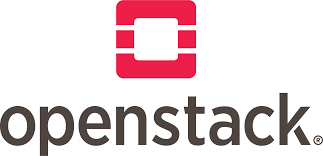
\includegraphics[scale=0.58]{openstack_logo}
 \caption{Openstack logo}
 \label{chap:prjan:img:openstack_logo}
\end{figure}

\subsubsection{Kubernetes}

As already introduced before, Kubernetes is an open source software framework
specialized in container management and orchestration. Developed by Google in
2014 and written in Go~\cite{k8sGit}, it allows different machines (called nodes
from now on) to create an abstraction layer and to form a cluster where is
possible to run Docker containers without bothering about hardware constraints.
Nodes can have specific roles and specialization, all of them managed by one or
many master nodes, that actually manage the orchestration. On top of that,
Kubernetes is virtualization-agnostic, meaning that it offers the possibility to
change the virtualization software in use (i.e. from Container-based technology
to Virtual machine software).
\begin{figure}[h]
 \centering 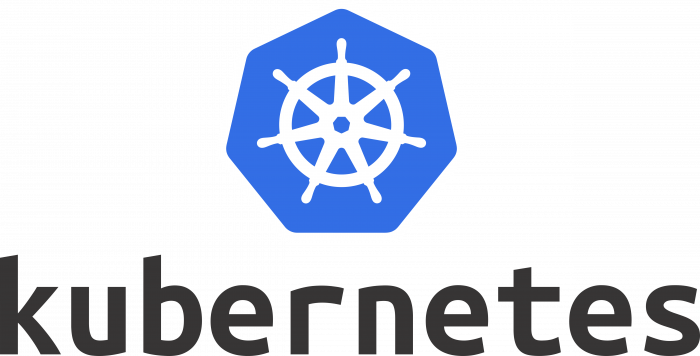
\includegraphics[scale=0.35]{kubernetes_logo}
 \caption{Kubernetes Logo}
 \label{chap:intro:img:k8s_logo}
\end{figure}


\subsubsection{Docker}

In recent years, with the new hardware capabilities and the recent development
of in-kernel virtualization systems (such as Hyper-V) this technology begin to
be adopted. Virtualization allows to run different systems on the same machine,
making them completely isolated and then more resilient to failures. The back of
the medal, though, is that virtual machines require large amount of resources,
especially memory, because solutions like copy-and-write of in-memory pages are
not viable anymore (since the kernel gets duplicated too), leading to
duplication of loaded libraries and assets in the memory of the host. For large
deployment containing only simple services (e.g. a back-end application serving
a website or a database) this ends up in a waste of resources. \todo{Talk about
  lxc containers and how Docker solved magically the problem.} It is here that,
in 2013~\cite{dockerWebsite}, Docker was created, basing its solution on an
already existing product: Linux Container (LXC). From this framework, Docker
built an entire ecosystem, consisting in a client/server model giving the
possibility for users to simply launch, scale and delete containers (locally or
remotely with Docker-machine), a repository system where images, a layer-based
``core'' where containers start running from when they are launched, can be
stored and tagged in a sort of version control system. Finally, another couple
of solutions, called Docker-compose, and Docker Swarm have the purpose to,
respectively, orchestrate containers in a single or a clustered system.
\begin{figure}[t]
 \centering 
\includegraphics[scale=0.7]{docker_logo}
 \caption{Official Docker logo}
 \label{chap:intro:img:docker_logo}
\end{figure}

\vspace{0.5cm}

% The development of the ETSI MANO test-bed involved the use of several 
% tecnhologies already in the market, and in some cases the creation of ad-hoc 
% solutions to solve particular issues. Here, a brief listing of the 
% well-estabilished technologies used is performed, describing even solutions 
% that at the end weren't chosen because they didn't fit with the defined goals.

\subsection{MANO}

Another fundamental component in the architecture is the MANO, that has to 
manage the Network Services and the deployment of new VNFs. In coordination 
with Kubernetes, it composes the core of the test-bed architecture. Initially 
identified with Openbaton (the component is described later 
in~\ref{chap:prjan:sec:tech:sub:other:sub:openbaton}), afterword it has been 
discovered to be not flexible enough to support other kinds of virtualization 
techniques than pure or in-cloud virtual machines\todo{Rewrite this}. 
Since this was a strong project requisite that could not be easily changed, it 
has been decided to opt for the creation of a smaller and simpler clone that 
offered a full integration with Docker and Kubernetes.

\subsubsection{Harbor}
\label{chap:prjan:sec:tech:sub:MANO:sub:harbor}
Started as a VNFM (Virtual Network Function Virtualization Manager) to offer a
bridge for Openbaton to interact with Kubernetes, during the project it has been
expanded to become a complete replacement of the original product, adding the
possibility to manage Network Services and to update the routing tables
contained in the Roulette Controller (the tool description can be found below
in~\ref{chap:prjan:sec:tech:sub:SFC:sub:roulette}). Harbor doesn't have a web
interface, but it has a RESTful API that allows users to interact with it using
CRUD operations. It offers functionalities similar to Openbaton: possibility to
save and retrieve VNF and NS definitions (basically, Kubernetes YAML
deployments). When an NS is saved, a consistency check is performed to assure
that all the VNFs have already been defined in Harbor. On an NS deployment, with
a mechanism similar to the Openbaton one, all the associated VNFs are set up
too, making the whole operation of launching a NS atomic from the user
point-of-view. What Openbaton doesn't do is a smart resource utilization:
Harbor, in fact, during a NS deletion, it checks if any related VNF remains
orphan (which means without any NS using it). In that case the VNF will enter in
a state of pruning: after five minutes, if the VNF has not be re-utilized by any
other NS it will be deleted. This mechanism assure faster deployments in
environments where NSs are continuously taken up and down. \todo{I've made an
  Harbor implementation schema, I dunno if its useful to put it here}

\subsection{SFC}
The tools analysis revealed little about already existent VNF or NS
implementations, so it was necessary to fill the gap. Since this one of our
thesis goals, we developed a complete solution to create a complete SFCs, trying
to standardize our vocabulary as much as possible, and giving basic
documentation when possible.

\subsubsection{Roulette Controller}
\label{chap:prjan:sec:tech:sub:SFC:sub:roulette}
Dynamic communications between VNFs would not be possible without a third
component acting as a route controller. Roulette fulfills this role, providing a
back-end where the single VNF can ask the next packet hop. Indeed, routes must 
be
submitted by another component, that we identified as Harbor (component
description available above in
sub-section~\ref{chap:prjan:sec:tech:sub:MANO:sub:harbor}). After a NS
deployment, Roulette gets instructed with a new route describing a NS. Every NS
has a proper ID (called \verb!sfid!), and thus when the classifier checks a
packet typology, it labels that packet with the specific NS ID (for a detailed
description about the SFC header see Section~\todo{Add section/chapter/paragraph
  ref!}). Finally, thanks to this label, every VNF knows the packet's chain and
it will correctly forward the it to the next VNF.

\subsubsection{Astaire}
As is possible to denote, a VNF doesn't only process the incoming packets, 
but it has to manage the communications and the related forward operations. To 
possibly ease part of the transmission problem and to make it easier to create 
a 
VNF without requiring the whole knowledge about SFC, it has been decided to 
build a framework, Astaire, that could keep the SFC related details decoupled 
from the core of the VNF, in other words, the entity that actually elaborates 
the packet. Built using an event-based pattern, it presents hooks that allow 
other software written in different languages from the Astaire one (e.g. Java), 
to be called dynamically at runtime in order to process the packet. The result 
of this elaboration gets returned to Astaire, that performs the beforehand 
cited operations of VNFs communications and forwarding.

\subsubsection{Ironhide}
As described in chapter~\ref{chap:archimpl}, the whole framework need to have 
and entry and an exit point. These, defined as \textit{Ingress} and 
\textit{Egress} points, are performed by Ironhide. Ironhide acts like a proxy, 
hiding the whole packet processing to the sender $S$ and the receiver $R$. When 
a client $S$ performs a request to $R$, the packet actually goes through 
Ironhide, who has an internal classifier that it is able to recognize the type 
of connection and to choose the right NS the packet has to go through. This 
process in fundamental since it keeps the connection between $S$ and $R$ up, 
for both TCP and UDP based communications.

\subsection{Technologies used during development}

Since the test-bed is composed by different components and thanks to its 
modularity, the implementation of the single components has been done with the 
help of additional tools, illustrated below

\subsubsection{Docker-compose} 
Docker-compose is a tool that allows services orchestration. It automates most 
of the tasks that should be performed by hand when launching one or multiple 
docker containers. It's particularly useful when more containers have to 
interact 
together, because\todo{Write down docker-compose functionalities and describe 
the product a little bit} all the services rules are described in a simple 
YAML file. With the birth of Docker Swarm, work has started to port this tool 
to 
the Swarm framework. At the time of this writing, the procedure to port a 
Docker-compose configuration in Docker Swarm (which a description of the 
product can be found in 
sub-section~\ref{chap:prjan:sec:tech:sub:other:sub:swarm}) is still not 
completely transparent, and it requires a sort of compilation, where 
Docker-compose bundles all the necessaries resources into a binary file that 
Docker Swarm will use to allocate the necessary resources.

\subsection{Other technologies evaluated}

Additional components have been evaluated during the development of the 
test-bed, and here we propose a list of the most important ones. Some of them 
where discarded as no more necessary, or during the evolution of the project 
itself they have become obsolete.

\subsubsection{Docker Swarm}
\label{chap:prjan:sec:tech:sub:other:sub:swarm}
Introduced in 2014~\cite{swarmGit}, Docker Swarm allows multiple Docker nodes to
cluster together and be seen as one logical unit. This layer completely makes
the underlying infrastructure transparent: data management, as network one, are
totally managed by Docker. Recently, Docker-compose support has been introduced,
making this one-node tool available for clustered systems. At the end of the
day, on one hand Docker Swarm provides an easy way to set up a cluster system
with all the tools configured out-of-the-box, without the necessity to set
networking configurations or installing ad-hoc storage solutions. On the other
hand, though, it doesn't have all the customization options that Kubernetes
offers, thus making the product less flexible. This fundamental characteristic,
although, makes the two solutions have different use cases leading to different
market needs.

\subsubsection{OpenVSwitch}
Started in 2009~\cite{ovsGit}, the OpenVSwitch project aims to create an
open-source multi-layer virtual switch. It provides a switching stack for
hardware virtualization environments, implementing several interfaces and
protocols. It has also the possibility to run through Hypervisor virtualization
but it can run under Docker too~\cite{ovsDocker}. OpenVSwitch can route packets
from incoming connections following rules, that can be ``pushed'' in its routing
table from software defined as \textit{controllers}. Additionally, it supports
the OpenFlow communication protocol, in order to set previously cited routing
definitions.

\subsubsection{Floodlight}
\label{chap:prjan:sec:tech:sub:other:sub:floodlight}
Community-developed and open source, Floodlight is an OpenFlow Controller
written in Java at the end of 2011~\cite{floodlightGit}. It allows various
applications to run on top of it. Floodlight has the role of controlling and
inquiring an OpenFlow network, querying the applications integrated with the
purpose of solving different user needs over it. When instantiated, OpenVSwitch
routers have to register to the controller in order to gain routing rules.


\subsubsection{Openbaton}
\label{chap:prjan:sec:tech:sub:other:sub:openbaton}
Patronized by the Institute Fraunhofer, it is an open-source, customizable NFV
MANO-compliant framework, that offers many configurations options, and since
it's written in Java, there is the possibility to add components (plug-ins)
dynamically. Openbaton can be installed as a normal computer program (they offer
packages for the most common distros) but it can be deployed on Docker
containers too. It's designed to work with cloud providers like Amazon or Google
Compute engine, but it offers compatibility with on-premise cloud solutions like
Openstack, where it deploys virtual machines using the API the platform offers.
It can store VNF configurations saved as Topology and Orchestration
Specification for Cloud Applications (TOSCA) Yet Another Markup Language (YAML)
and it can handle multiple Point of Presence (PoP). It offers a VNF lifecycle
management out-of-the-box, with the possibility to customize it based on the
user needs. Its modular design allows developers to change parts of the codebase
with custom ones, making the product really flexible to different platforms.
Performing this operation requires a deep knowledge of the framework though.
\begin{figure}[h]
 \centering 
\includegraphics[scale=0.45]{openbaton_logo}
 \caption{Openbaton logo}
 \label{chap:prjan:img:openbaton_logo}
\end{figure}
